% --- Section: Methodology ---
% Drafted Phase 6 — values pulled from cleanup/04_phase5_data_pulled.md
% and canonical sources (code/data_preprocessing/, code/analysis/, code/models/).
% Target: ~700 words.

\section{Methodology}
\label{sec:methodology}

\subsection{Task Suite}

171 base tasks across 38 task types, split into two phases.
Phase~1 (136 tasks, 31 types) covers closed-form conjugate
Bayesian models: Beta--Binomial, Gamma--Poisson, Normal mean with
known and unknown variance (Normal--Inverse-Gamma),
Dirichlet--Multinomial, Bayesian linear regression, and
decision-theory tasks (Bayes risk under squared, absolute, and
0--1 loss). Phase~2 (35 tasks, 7 types, 5 tasks each) covers
computational Bayesian methods: Gibbs sampling,
Metropolis--Hastings, Hamiltonian Monte Carlo, Reversible-Jump
MCMC, hierarchical models, Variational Bayes, and Approximate
Bayesian Computation. Every task has a ground-truth solver
implemented from
textbooks~\cite{bolstad2007bayesian,hoff2009bayesian,bishop2006prml}.
Phase~2 stochastic methods use seeded Monte Carlo estimates as
ground truth, with tolerances of 0.05 for MCMC variants and 0.10
for VB and ABC.

\begin{figure}[!ht]
  \centering
  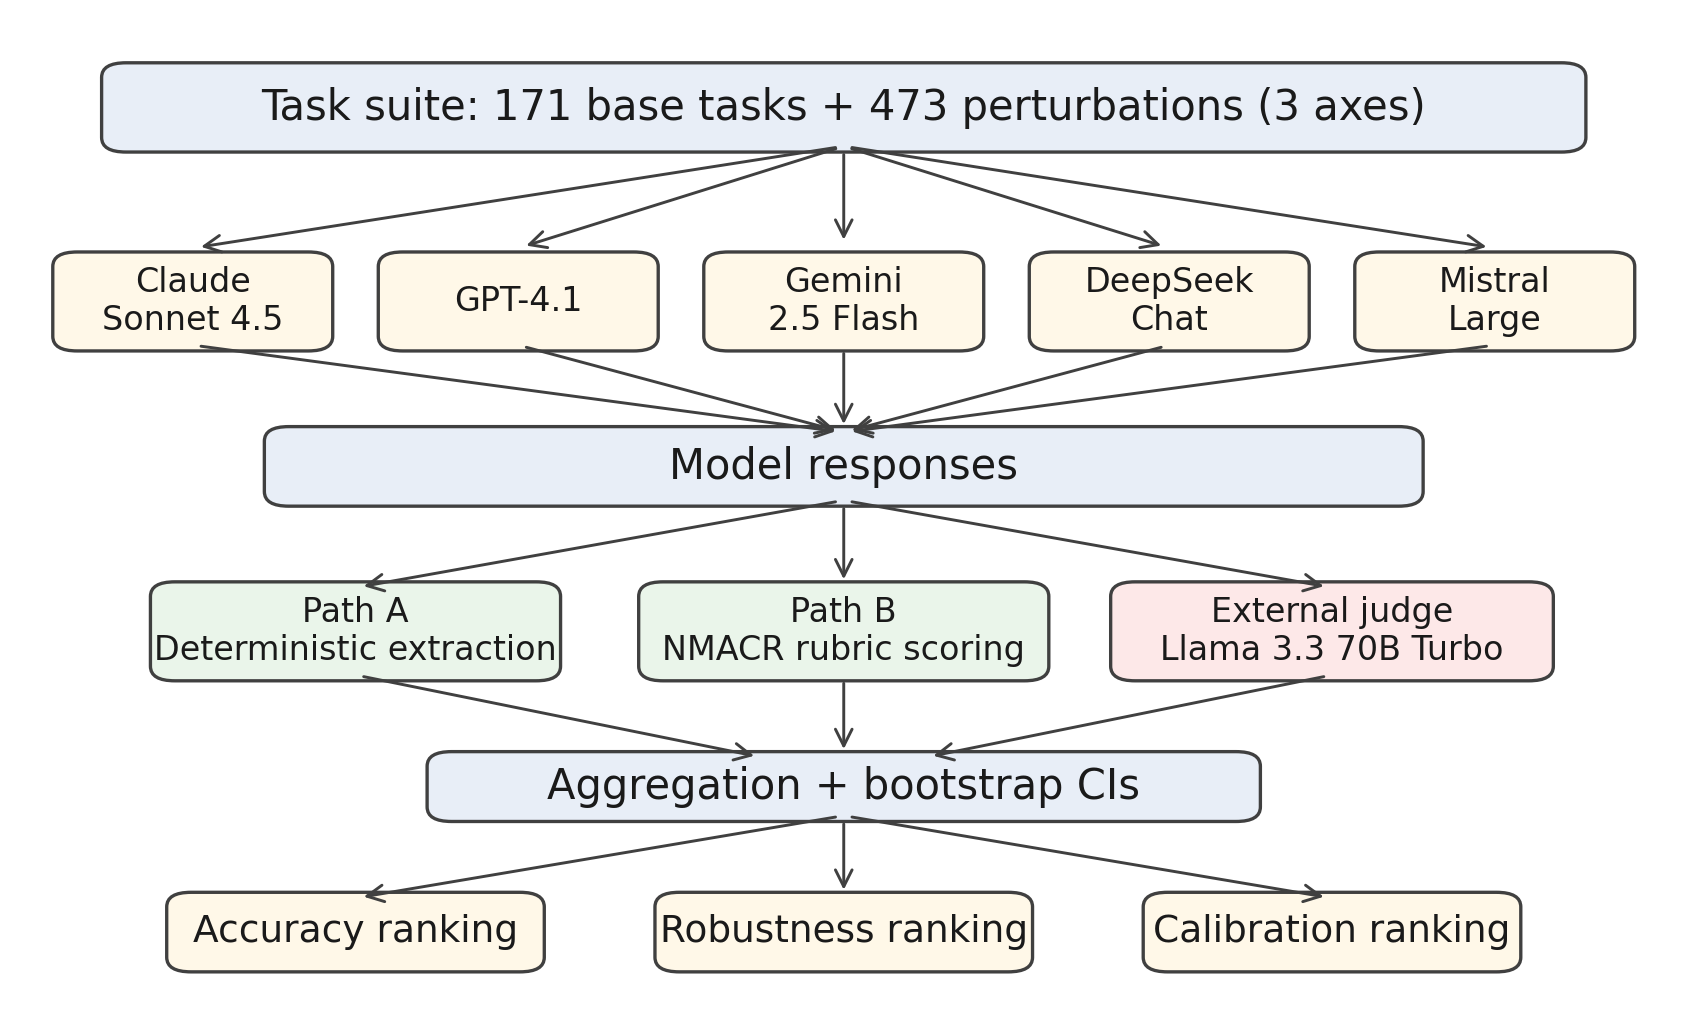
\includegraphics[width=\columnwidth]{figures/pipeline.png}
  \caption{Evaluation pipeline. Each task and its perturbations are
           passed to five frontier LLMs in parallel. Responses are
           scored via three independent paths: deterministic extraction,
           NMACR rubric scoring, and an external Llama 3.3 70B judge
           for assumption-compliance. Aggregated scores yield three
           independent rankings.}
  \label{fig:pipeline}
\end{figure}

\subsection{Perturbation Taxonomy}

Each base task is perturbed along three axes. \emph{Rephrase}
preserves the math and the answer while rewording the prompt.
\emph{Semantic} preserves the math while relocating the problem
to a different real-world framing. \emph{Numerical} changes the
numerical inputs and recomputes the ground-truth answer. The full
set contains 473 records: 75 hand-authored seeds covering 25 base
tasks across all three axes, and 398 LLM-generated perturbations
covering the remaining 146 base tasks, produced by the same Llama
3.3 70B Turbo used as the assumption-compliance judge. Every
LLM-generated perturbation was checked against the ground-truth
solver before inclusion. Mean coverage is 2.77 perturbations per
base task. The numerical axis is skipped for 40 conceptual or
seeded-MC tasks where swapping numbers would invalidate the
ground-truth procedure.

\subsection{Three-Path Scoring}

Each response is scored three ways. \textbf{Path~A} is a
deterministic keyword rubric in the live runner. It extracts the
answer line, compares numeric targets to the ground truth within a
per-task tolerance, and checks required structural and assumption
keywords in the free-form prose. \textbf{Path~B} is a post-hoc
NMACR aggregator. Each task contributes five components in
$[0,1]$: numerical accuracy (N), method structure (M), assumption
compliance (A), confidence calibration (C), and reasoning quality
(R). The combined score is a weighted sum,
\begin{equation}
  S_{\text{NMACR}} = 0.10\,N + 0.20\,M + 0.30\,A + 0.15\,C + 0.25\,R,
  \label{eq:nmacr}
\end{equation}
with weights drawn from the chain-of-thought, calibration, and
assumption-articulation
literature~\cite{wei2022cot,chen2022pot,guo2017calibration,du2025icecream,park2025judge,nagarkar2026canllm,fermieval2025,liu2025matheval}.
A gets the highest weight because assumption articulation is what
Bayesian reasoning is for; N gets the lowest because a correct
number with no derivation does not answer the question. Pass
threshold is $s \geq 0.5$. \textbf{Path~C}, the external judge,
runs on one dimension only. Each (task, response) pair is sent to
Llama 3.3 70B Turbo via the Together AI API with a fixed rubric
prompt asking whether the response explicitly states the
assumptions the task requires. The narrow scope is a direct
response to the holistic-judge failure modes that Feuer et
al.~\cite{judgment2025noise} document.

\subsection{Three-Ranking Framework}

We compute three rank orders from the same response corpus. The
\emph{accuracy ranking} uses the Path~B NMACR pass rate per model
across all 171 base tasks. The \emph{robustness ranking} uses the
perturbation pass-flip rate. Let $\mathrm{pass}(t, m) \in \{0,1\}$
be the binary base pass for task $t$ and model $m$, and
$\overline{\mathrm{pass}}(t, m)$ the mean pass over $t$'s
perturbations $\mathcal{P}(t)$. The model's robustness is
\begin{equation}
  R_m = 1 - \frac{1}{|\mathcal{T}|}\sum_{t \in \mathcal{T}}
        \left| \mathrm{pass}(t, m) - \overline{\mathrm{pass}}(t, m) \right|,
  \label{eq:robustness}
\end{equation}
with $R_m = 1$ for perfect base/perturbation agreement. Bootstrap
CIs use 10{,}000 non-parametric resamples (seed 42). The
\emph{calibration ranking} uses binary-pass Expected Calibration
Error~\cite{guo2017calibration} over $B$ confidence buckets,
\begin{equation}
  \mathrm{ECE} = \sum_{b=1}^{B} \frac{|B_b|}{N}
                 \,\bigl|\,\mathrm{acc}(B_b) - \mathrm{conf}(B_b)\,\bigr|,
  \label{eq:ece}
\end{equation}
where $B_b$ is the set of predictions in bucket $b$,
$\mathrm{acc}(B_b)$ is empirical accuracy within the bucket, and
$\mathrm{conf}(B_b)$ is the bucket's mean confidence. We use
$B = 4$ buckets (low, medium, high, unstated) parsed from the
response's hedging language. The three rankings are not redundant:
a model can be accurate but brittle, accurate and well-calibrated
but brittle, or robust but inaccurate. \S\ref{sec:results} shows
all three of those configurations actually occur in our five-model
sample.

\subsection{Experimental Setup}

\textbf{Models and APIs.} The five LLMs are queried directly over
their HTTP APIs with no vendor SDKs: Claude Sonnet 4.5 (Anthropic
Messages), GPT-4.1 (OpenAI Chat Completions), Gemini 2.5 Flash
(Google Generative Language), DeepSeek-Chat, and Mistral Large.
Decoding settings are the same for every provider. Temperature
is the API default (around 1.0 for the chat endpoints). Max
output is 1024 tokens. Each call has a 60-second timeout and
retries on transient 429 and 5xx responses. The same
Bayesian-statistics system prompt is used for every model.

\textbf{Evaluation pipeline.} Each (task, model) pair produces
one response. Path~A extracts the final answer line and structural
keywords. Path~B aggregates the five NMACR components into a
weighted score. The external Llama 3.3 70B Turbo judge, served by
Together AI's OpenAI-compatible API, scores the response on
assumption-compliance only. Perturbations go through the same three
paths. Single-pass per (task, model) is the default; a small
self-consistency subset (3 samples) is used for the calibration
analysis.

\textbf{Calibration computation.} Equation~\ref{eq:ece} is
computed per model on the full response corpus. Uncertainty is
reported as 95\% percentile bootstrap confidence intervals over
10{,}000 non-parametric resamples of per-run aggregate scores
(seed 42), the same procedure used for the accuracy and robustness
CIs.

\textbf{Reproducibility.} A single shell script drives the full
pipeline: deduplication, scoring, perturbation scoring, judge
invocation, and aggregation. 53 unit tests cover the task
generators and the MCP query interface. Every figure in the paper
is generated by the R analysis pipeline at
\emph{report\_materials/r\_analysis/run\_all.R}; none are
hand-edited.
